	% Journal Article
% LaTeX Template
% Version 1.4 (15/5/16)
%
% This template has been downloaded from:
% http://www.LaTeXTemplates.com
%
% Original author:
% Frits Wenneker (http://www.howtotex.com) with extensive modifications by
% Vel (vel@LaTeXTemplates.com)
%
% License:
% CC BY-NC-SA 3.0 (http://creativecommons.org/licenses/by-nc-sa/3.0/)
%
%%%%%%%%%%%%%%%%%%%%%%%%%%%%%%%%%%%%%%%%%

%----------------------------------------------------------------------------------------
%	PACKAGES AND OTHER DOCUMENT CONFIGURATIONS
%--------------%%%%%%%%%%%%%%%%%%%%%%%%%%%%%%%%%%%%%%%%%
%--------------------------------------------------------------------------

\documentclass[twoside,onecolumn]{article}

\usepackage{blindtext} % Package to generate dummy text throughout this template 

\usepackage[sc]{mathpazo} % Use the Palatino font
\usepackage[T1]{fontenc} % Use 8-bit encoding that has 256 glyphs
\linespread{1.05} % Line spacing - Palatino needs more space between lines
\usepackage{microtype} % Slightly tweak font spacing for aesthetics

\usepackage[english]{babel} % Language hyphenation and typographical rules

\usepackage[hmarginratio=1:1,top=32mm,columnsep=20pt]{geometry} % Document margins
\usepackage[hang, small,labelfont=bf,up,textfont=it,up]{caption} % Custom captions under/above floats in tables or figures
\usepackage{booktabs} % Horizontal rules in tables
\usepackage{graphicx}
\usepackage{lettrine} % The lettrine is the first enlarged letter at the beginning of the text

\usepackage{enumitem} % Customized lists
\setlist[itemize]{noitemsep} % Make itemize lists more compact

\usepackage{abstract} % Allows abstract customization
\renewcommand{\abstractnamefont}{\normalfont\bfseries} % Set the "Abstract" text to bold
\renewcommand{\abstracttextfont}{\normalfont\small\itshape} % Set the abstract itself to small italic text

\usepackage{titlesec} % Allows customization of titles
\renewcommand\thesection{\Roman{section}} % Roman numerals for the sections
\renewcommand\thesubsection{\roman{subsection}} % roman numerals for subsections
\titleformat{\section}[block]{\large\scshape\centering}{\thesection.}{1em}{} % Change the look of the section titles
\titleformat{\subsection}[block]{\large}{\thesubsection.}{1em}{} % Change the look of the section titles

\usepackage{fancyhdr} % Headers and footers
\pagestyle{fancy} % All pages have headers and footers
\fancyhead{} % Blank out the default header
\fancyfoot{} % Blank out the default footer
\fancyhead[C]{PAYSURA $\bullet$ December 2017 $\bullet$ Whitepaper} % Custom header text
\fancyfoot[RO,LE]{\thepage} % Custom footer text

\usepackage{titling} % Customizing the title section

\usepackage{hyperref} % For hyperlinks in the PDF

%----------------------------------------------------------------------------------------
%	TITLE SECTION
%----------------------------------------------------------------------------------------

\setlength{\droptitle}{-4\baselineskip} % Move the title up

\pretitle{\begin{center}\Huge\bfseries} % Article title formatting
\posttitle{\end{center}} % Article title closing formatting
\title{PAYSURA} % Article title
\author{%
\textsc{The International PayReward Coin (IPC)} \\[1ex] % Your name
\normalsize \href{mailto:contact@paysura.com}{contact@paysura.com} % Your email address
%\and % Uncomment if 2 authors are required, duplicate these 4 lines if more
%\textsc{Jane Smith}\thanks{Corresponding author} \\[1ex] % Second author's name
%\normalsize University of Utah \\ % Second author's institution
%\normalsize \href{mailto:jane@smith.com}{jane@smith.com} % Second author's email address
}
\date{December 24, 2017} % Leave empty to omit a date
\renewcommand{\maketitlehookd}{%
\begin{abstract}
\noindent
An abstract look at the world's economic and financial system specifically shows that it is driven by producers and consumers, or supply and demand: the products offered match consumers' demand. The consumer pays for a product and receives ownership of it or the right to use it. This system generates several essential difficulties in example for online and offline merchants and their consumers in particular. Merchants face the problem of customer retention whereas customers often don't benefit from being loyal to specific merchants over a certain period of time. In order to solve these problems for both merchants and customers many different companies introduced individual or overarching customer gratification systems such as \textit{Payback} etc. And although customer gratification systems are a great idea, widely accepted and widespread internationally the contemporary approach comes along with several new and so far unsolved issues. These gratification systems resemble costly liabilities for the merchants and customers face problems such as a rewards jungle of thousands of different reward programs, limited usability options, plastic cards and data security etc. PAYSURA is aware of these problems therefore introducing the International PayReward Coin (IPC) in order to establish a worldwide available, uniform and secure reward system that applies the advantages of the blockchain technology.



% Dummy abstract text - replace \blindtext with your abstract text
\end{abstract}
}

%----------------------------------------------------------------------------------------

\begin{document}

% Print the title
\maketitle

%----------------------------------------------------------------------------------------
%	ARTICLE CONTENTS
%----------------------------------------------------------------------------------------

\section{Introduction}

\lettrine[nindent=0em,lines=3]{P}AYSURA is providing the International PayReward Coin (IPC). IPC is a coin that rewards 
customers for buying products or services. The focus of IPC is to be available worldwide as a uniform and secure reward system through the blockchain technology.\\
No tracking of customer data or influence on consumer behavior due to the Ethereum blockchain. No complicated registrations. No physical cards to be held in the personal wallet. No expiration dates for the use of the IPC. PAYSURA is providing the only reward system which is modern, secure and available worldwide through the blockchain. The customer has full control over his collected reward in IPC, and will be able to send or transfer these to friends, family members or colleagues throughout the world. 
Customers will be able to collect IPC through different channels and options. One will be to embed IPC on different platforms where products such as smartphones, TVs or services such as video-on-demand, insurance or even car sharing packages can be bought. Reward in IPC will be generated through these platforms and automatically sent to the customer. 
Other options will be the cryptocurrency market in general as well as partner programs that reward customers by IPC. Partner programs with car manufacturers will be established, allowing customers to purchase a car and earn reward for the purchase in IPC. All IPC can be used in a reward pool provided by PAYSURA to exchange collected values for real values. 


%------------------------------------------------ PAYSURA is providing the International Payback Coin (IPC) as a reward for customers buying new products or services. The concept is simple: The consumer is looking for a new product, the consumer will register on the PAYSURA platform, the consumer will select his product, the consumer will buy his product and he will receive IPCs automatically. No complicated configuration, no confusing installments, just a simple registration. The platform of PAYSURA will be easy to manage for everyone and no previous knowledge about cryptocurrencies will be required. The gained IPCs will be stored automatically in an automated generated address after the registration. Neither the consumer nor the supplier will have to handle any IPC configurations because all IPCs will be paid by PAYSURA. PAYSURA is rewarding every consumer and giving an asset to every consumer without any disadvantages for the supplier.



\newpage


\section{PAYSURA - The Business Model}

PAYSURA is introducing the International PayReward Coin (IPC). PAYSURA wants to provide a uniform reward and bonus system which is available worldwide, without using any physical cards which have to be carried in the customer's personal wallet. Currently, one physical card cannot be used in every shop or for every service - there are too many providers and therefore too many cards to be managed by the customer. PAYSURA will provide a blockchain based reward system. The blockchain will make it possible to offer IPC throughout the world and make it usable for everyone. Every merchant can use IPC as a reward system for his products. The consumer will receive these IPC by buying the product or by paying for a service of the merchant.
\\
PAYSURA has developed the COMD-Business Model - \textbf{C}ustomer \textbf{O}riented not \textbf{M}erchant \\
\textbf{D}isadvantaging (\textbf{COMD}). 
The COMD-Model consists of three parties - Merchant, Administrator, Customer - and one value - the Reward.

\begin{itemize}
\item The Reward:
\end{itemize}
The reward in this Concept will be IPC. IPC is a coin and the key to an international reward system that can be used by every customer and merchant worldwide. In the COMD-Model the reward is the key player and the circulating factor of the whole model. The IPC will be issued by PAYSURA during the crowdsale while some of the IPC will be reserved for the reward system. IPC can be collected through a merchant who offers any kind of product or service and works with the PAYSURA reward system. PAYSURA will handle the configuration for every merchant and offer APIs to all merchants so that it will be possible to use the self-regulated reward algorithms developed by PAYSURA. The reward will be sent to the customer automatically after a successful purchase has been processed. The IPC can also be used in the PAYSURA reward pool to receive real values for the collected IPC. No physical cards are necessary to receive IPC. The customer will register at PAYSURA, automatically generating a wallet into which all IPC which are received during a purchase will be transferred.\\
PAYSURA wants to integrate a reward into every possible product such as electronics, retail or services like video-on-demand, car sharing, taxi rides, insurance, car dealers and many more. The goal is to generate reward for every transaction where money is paid for any kind of value or good. 

\begin{itemize}
\item The Customer:
\end{itemize}
The customer is the asset player of the whole concept. The COMD-Model is a customer oriented model that implies a concept focused on the customers' advantages and extending these as much as possible. The customer will be the receiver of the value or reward in terms of IPC. In buying a car, purchasing new shoes, or using a paid service, the customer will receive IPC and be rewarded for his purchase. The customer will receive his IPC automatically and can use these in the PAYSURA reward pool to exchange them for real products or values. The customer can also participate in the selection of the products in the reward pool. The whole model is mainly focused on the customer and using his demands to utilize the whole capability of the COMD-Business Model. 

\begin{itemize}
\item The Merchant:
\end{itemize}

The COMD-Model is a customer-oriented but not a merchant disadvantaging business model. The main question that arises is about the payment of the IPC. Who is paying the IPC that are used as reward? The answer is a non-loss principal using the commission system. A merchant offers a product through some kind of mediator, e.g. Daimler produces a Mercedes-Benz E Class which is offered by many mediators. When a car is sold, the vendor earns a commission and Daimler receives the sales price. This is a winning situation for both sides. The COMD-Model introduces a similar system for the merchant using IPC. The difference is that the commission for an offered product will be used and a part will be used as reward. Through the blockchain technology and the worldwide range of the community that can use IPC many costs will be saved, making it possible to bring a substantial reward amount to the customer. Imagine a salesman selling a car for around \$30,000 and earning a commission of 10\%, which comes out to \$3,000. As the blockchain technology will allow many costs to be saved, it will be possible to return a large portion of IPC to the customer. This will allow a merchant to gain many more customers, growing his organization without decreasing his income. The value transferred to the customer through the COMD-Model will increase the visibility of a merchant's products or services without any disadvantages. The whole regulation and implementation will be done by the administrator of the COMD-Model. 
\begin{itemize}
\item The Administrator:
\end{itemize}

In the COMD-Business Model PASYURA is the administrator. The administrator will provide interfaces for communication between merchant and customer and the transferred values. PAYSURA will implement a self-regulated reward system and offers an interface for every merchant to include the reward system so that the transfer of the IPC to the customers will be self-automated. Using blockchain technology, PAYSURA will be able to implement the reward in terms of IPC everywhere in the world; small startups or big companies can use IPC with the same basis. \\
\\
COMD is a future-proof business model acting independently of any technical issues with the focus on the customers' demand and assets. 

\begin{figure}[ht]
\centering
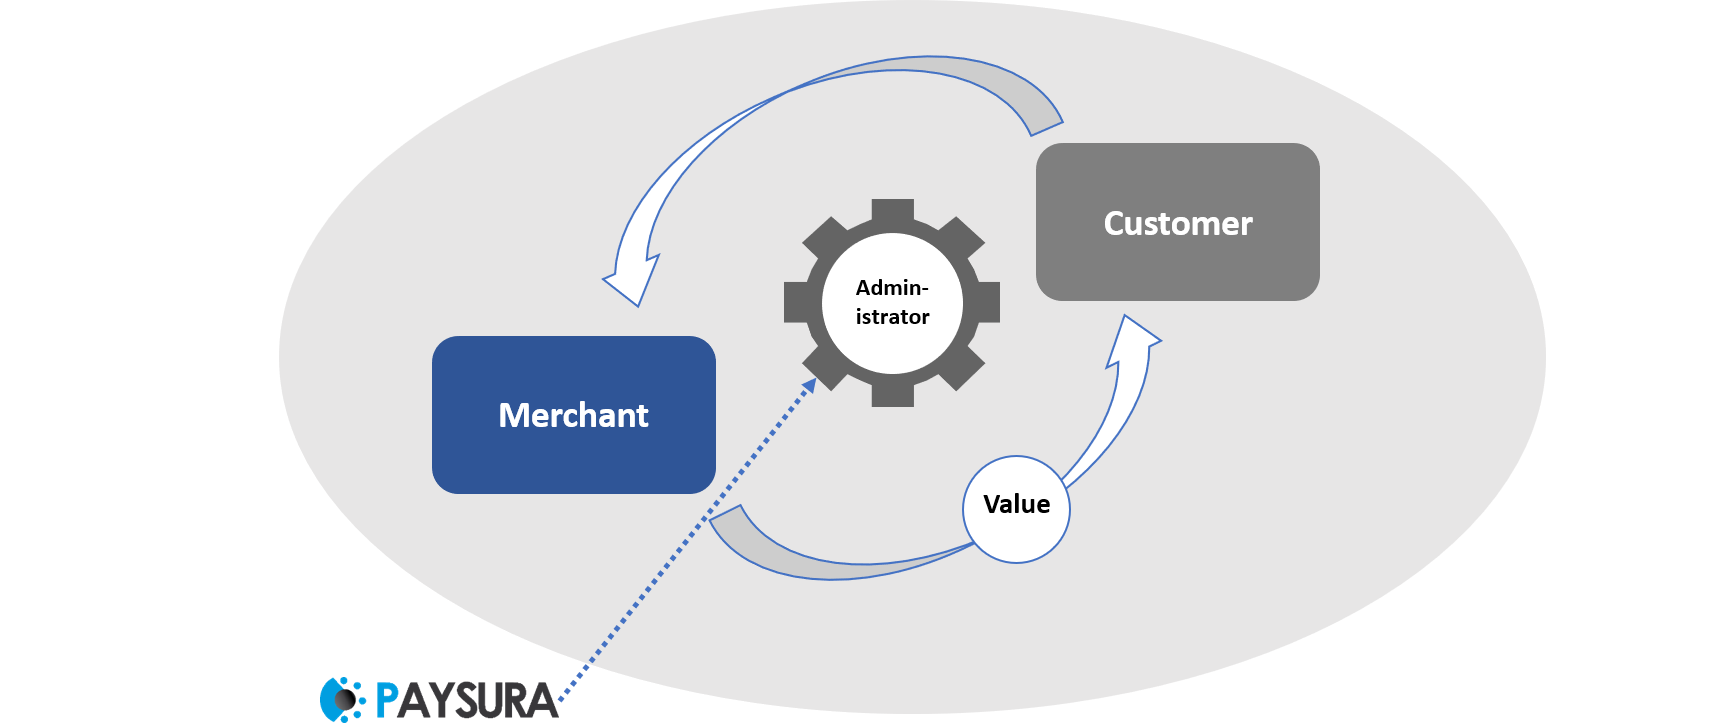
\includegraphics[scale=0.34]{COSD_modell23.png}
\caption{PAYSURA - The COMD-Business Model}
\label{pool}
\end{figure}

\begin{table}[ht]
\centering
\label{my-label}
\begin{tabular}{lll}
                                           & Commercial Reward/Cashback & PAYSURA-IPC \\
Reward Program                             & Yes                         & Yes         \\
Exchange Points for Values                 & Yes                         & Yes         \\
Available Worldwide                        & No                         & Yes         \\
Uniform                                    & No                          & Yes         \\
Secure                                     & No                          & Yes         \\
Physical Card/Bonus Card                   & Yes                         & No         \\
Automated \& Self-Regulated Reward System & No                          & Yes         \\
Time Limit/Expiration of Collected Reward & Yes                         & No         
\end{tabular}
\caption{Comaprison of conventional Reward/Cashback Systems vs. PAYSURA}
\end{table}
\newpage
\section{PAYSURA - Tiers and Components}

To establish an international reward system, a uniform concept with a modular structure is needed to allow it to be extended every time. Additionally, it needs to be available anytime and everywhere. This system will be adaptable for every partner or platform in a very easy way. Using blockchain technology, such a system can be built to create a reward token which will be available worldwide in a secured system, protected from any possible manipulation of the owned IPC. PAYSURA will implement a uniform, worldwide reward system to bring an asset to all customers. To this end, PAYSURA is starting a crowdsale where the implementation will be tiered in the following way:
\begin{itemize}
\item Funding of \$5,000,000 - \$15,000,000:
\end{itemize}
- Development of PAYSURAs Digital Reward Ecosystem\newline
- Developing PAYSURA inside and outside the organisation \newline
- Expanding team\newline
- Building sophisticated state of the art IT Infrastructure\newline
- Development and rollout of iOS, Android and Windows Mobile App\newline
- Enhance first markets marketing efforts\newline
- Development of Merchant integration into PAYSURAs Digital Reward Eco System \newline
- Development and rollout of the PAYSURA reward pool in the first market\newline
- Development and rollout of the IPC Wallet \newline
- Products mostly offered by major merchants partnering with PAYSURA\newline

\begin{itemize}
\item Funding of \$15,000,000 - \$30,000,000:
\end{itemize}
- Collect a data set to train an AI algorithm for the self-regulated reward system\newline
- Extend the self-regulated algorithm with AI functionialities \newline
- Products of the PAYSURA Reward pool will mostly be community driven and offered by PAYSURA \newline
- \textit{One touch} registration on the PAYSURA Plattform \newline
- Expand the PAYSURA reward system to the retail industry \newline
\\

The different components in detail:\\


\textbf{Reward Pool:}\\
The reward pool will be a web application where collected IPC can be exchanged for real values. This pool will offer partner products, services and selected products voted by the community. \\


\textbf{IPC:}\\
The International PayReward Coin (IPC) is an international token, available worldwide, which will be used as reward for a purchased product. Purchasing insurance, using a video-on-demand service or simply buying a new TV will generate IPC for the customer. The target is to establish IPC in every shop and on all platforms where services or products are purchased. Every merchant can offer IPC and use the PAYSURA's self-regulated reward system to offer IPC for his own products. IPC will be available through the blockchain worldwide and every merchant will be able to use it without security issues. The customer will not hold any physical card or any other kind of bonus cards. The customers' purchases will not be tracked. The collected IPC can be shared, sent or just held by the customer. There is no expiration date for the use of IPC in the reward pool. The integrated wallet on the PAYSURA application allows the easy exchange of IPC for a real product without complicated configurations. For security reasons a two-factor authentication will be implemented. \\



\textbf{PAYSURA Platform:}\\
PAYSURA's long-run, contribution dependent target is to establish its own platform for offering products or services. This platform will use the self-regulated reward system and all products offered by any merchant will automatically offer IPC. PAYSURA will take a commission for offered and sold products and will pay the reward amount in terms of IPC. This platform will guarantee support of the PAYSURA reward system. \\



\textbf{Service Concept:}\\
PAYSURA wants to bring the reward coin into every use case, whenever a payment is made. A future step of PAYSURA will be to bring IPC into different services such as the video-on-demand and car sharing market. The concept is to reward the user with IPC for watching movies or driving a car and paying money for it. In using such services, the customer gains IPC that can then be used in the reward pool and exchanged for products offered there. \\



\textbf{Partner Programs:}\\
PAYSURA will also focus on partnerships and forge different partner programs like insurance and automobile manufacturer to provide IPC. Many people enter into insurance contracts and pay an amount for a service that, in many cases, is never used. In a legal expense insurance contract, for example, the policy holder pays a monthly fee year after year, often without ever using the service. In such cases, PAYSURA wants to award customers with IPC annually, for new or extended insurance contracts. \\
The same use case can be applied to car sales. Customers pay large sums to buy a new car, for which the car salesman also receives a high commission. This situation presents many options to bring more value to the customer by using IPC as a reward system for the purchase of a new car.\\
\\
The International PayReward Coin (IPC) can be implemented in every use case where money is exchanged for a product or service. Paying rent for the flat, purchasing petrol or even paying for school books. In all these cases, a reward for the customer will be implemented by using the IPC. PAYSURA wants to envelop the market with IPC to generate more assets for customers. 








%------------------------------------------------
\section{PAYSURA - The car sharing example} 
Imagine Alex is 29 years old and lives in Berlin, Germany, working as an IT consultant. His job requires a lot of travel, and he is currently working in London, UK four times a week. In the first days, Alex uses a car sharing service to get an overview of the city. He notices that one car sharing company offers IPC as reward for using their service. Alex rents one car for two hours, and after his short trip through London he finishes his rental period and returns home. Some moments later, Alex gets a notification that he has received IPC for using the service. Alex is happy and decides to use the service much more to continue earning IPC.	 After a while Alex has collected a given amount of IPC and visits the reward pool. He is looking for a massage seat to use on his trips with the car sharing service. Alex exchanges his IPC and is now the owner of a new massage seat, making his drives much more comfortable.

%\section{PAYSURA - The Television Example}

%Imagine Alex, a supporter of the International Payback Coin. Alex is currently moving into a bigger flat and notices that his new %living room is much bigger than his old one. A bigger living room means a bigger TV. So Alex starts his research for an affordable %TV that will be large enough for his new living room. During the research he finds out that the prices are nearly the same in all %markets but then Alex notices the PAYSURA platform. The same TV is listed in the PAYSURA platform for the same price, but includes %an IPC reward for the purchase. Now Alex decides to buy this TV on the PAYSURA platform. In the first step Alex will go through a %registration process with general information. Afterwards Alex can select his TV and add it to his cart. Alex notices that it is %possible to pay for the TV with cryptocurrency. Alex likes this and decides to pay the amount in Ether. So Alex confirms the whole %process and buys the article. Alex now has 15 minutes to send his Ether to the given address. After his Ether transaction is %confirmed, PAYSURA will send a notification to Alex and Alex will be the owner of a new TV. His IPC will be sent to his integrated %wallet and Alex will see the balance of his IPC in his profile. Alex has bought a new TV and earned IPC in addition.
\section{PAYSURA - The IPC Example}

After four years of use, Alex's old smartphone is no longer usable and he needs a new one. Alex notices that he has collected a lot of IPC, so he decides to visit the PAYSURA reward pool to look for a suitable smartphone that meets his demands. Alex can filter for smartphones and see all those available for his current amount of IPC. After selecting a smartphone Alex can simply click on exchange and confirm the exchange. Alex IPC will be transferred automatically to PAYSURA and the smartphone will be sent to Alex. The IPC Alex has sent to PAYSURA can now be used for other products as reward and Alex has purchased a brand new smartphone.

%\begin{figure}[ht]
%\centering
%\includegraphics[scale=0.4]{payback_pool.png}
%\caption{PAYSURA - An illustration of the Reward Pool}
%\label{pool}
%\end{figure}
%\clearpage



%\section{PAYSURA - The first step: Insurances}

%At the beginning, PAYSURA will focus on the insurance industry.
%The focus in this branch is to deliver an asset for customers who take out new insurance policies and pay monthly or annual fees, %often without ever using the whole capacity of the agreement. PAYSURA is paying attention to this issue and will elaborate a %situation in which an asset can be generated for a customer with insurance.
%After registration with an insurance company, the customer will be able to receive IPC as reward. For each policy, the customer %will receive a signing bonus and an annual reward paid directly to the customer in IPC. The following two use cases further %demonstrate the insurance concept:
%\begin{itemize}
%\item	Imagine Steve, who is already familiar with cryptocurrencies and can make use of the crowdsale to earn IPC. He can then use them in the reward pool and exchange them for other products or services. For example, Steve needs car insurance with costs a monthly fee of \$50. For this insurance, he will gain 5 IPC and additionally earn an annual reward offered individually by the insurance company. He can use the IPC earned through his insurance policy to purchase goods or services from the reward pool.
%\item	The second use case is for users who are unfamiliar with cryptocurrencies or crowdsales. A registered insurance company will also have a local access to the PAYSURA platform so it can provide the reward system to customers. The insurance company will ask the customer if he would like to participate. If the customer agrees, some customer data will be transferred to PAYSURA. PAYSURA can now contact the customer and perform all configurations for the customer and transfer IPC to the customers wallet. \\ Additionally, the PAYSURA platform itself can be used to find a suitable insurance policy and earn IPC. The policies will be listed on the platform and the customer will see how many IPC he will receive for each insurance policy. The payment can optionally be made in cryptocurrency or fiat money.
%\end{itemize}
%The customer can always see his amount of IPC and its value compared to other cryptocurrencies.
%The target of PAYSURA is not only to focus on users who are familiar with cryptocurrencies. IPC should be available for every consumer who is in contact with insurance companies willing to use such a reward system. IPC will be a fully closed reward system based on the demand of the customer.\\
%In an upcoming step the target is the integration of third parties into the insurance concept of IPC. 
%One use case example with Steve:

%\begin{itemize}
%\item	Use case: Steve needs a lawyer due to a parking ticket.
%\item	What does Steve do? Steve will contact his lawyer and his legal insurance to pay his lawyer.
%\end{itemize}
%A future step will be to include the lawyer in this concept. Lawyers will also be able to offer IPC, allowing Steve to choose one %and gain IPC. Additionally, Steve's insurance can suggest a lawyer to him. If he chooses this lawyer, Steve will earn a given amount of IPC. Similarly, doctors, car service stations, and more can be integrated in the IPC system step by step.
%\clearpage
\section{PAYSURA - Crowdsale}
To establish an international reward system, a uniform concept with a modular structure is needed to allow it to be extended every time. Additionally, it needs to be available anytime and everywhere. This system will be adaptable for every partner or platform in a very easy way. Using blockchain technology, such a system can be built to create a reward token which will be available worldwide in a secured system, protected from any possible manipulation of the owned IPC. PAYSURA will implement a uniform, worldwide reward system to bring an asset to all customers.
The development of the PAYSURA platform and the reward pool needs a well-planned infrastructure which requires a large budget. Funding will be raised with a crowdsale where the community will receive IPC, which can then be exchanged for goods and services in the reward pool. PAYSURA will limit the capacity of IPC at 440 000 000 tokens where 60 \% (264 000 000) will be offered during the crowdsale, and 25 \% (110 000 000) will be reserved for the community as reward in the platform. This means 85 \% of IPC will be reserved and solely handed out to the community. The last 15 \% (66 000 000) are reserved for advisors and partners (5 \%), and the development and future progress of PAYSURA (10\%). 
PAYSURA wants to deliver assets to the community. In order to do this, 30\% of the funded amount will be reserved for products that will be available to the community in the reward pool.  70 \% of the funded amount will be used for the development of PAYSURA (see Figure \ref{dg1}) according to the tiers described above. Unsold IPC will be used for reward and therefore be offered to the community.
The crowdsale will run for 30 days with the following distribution program:

\begin{figure}[ht]
\centering
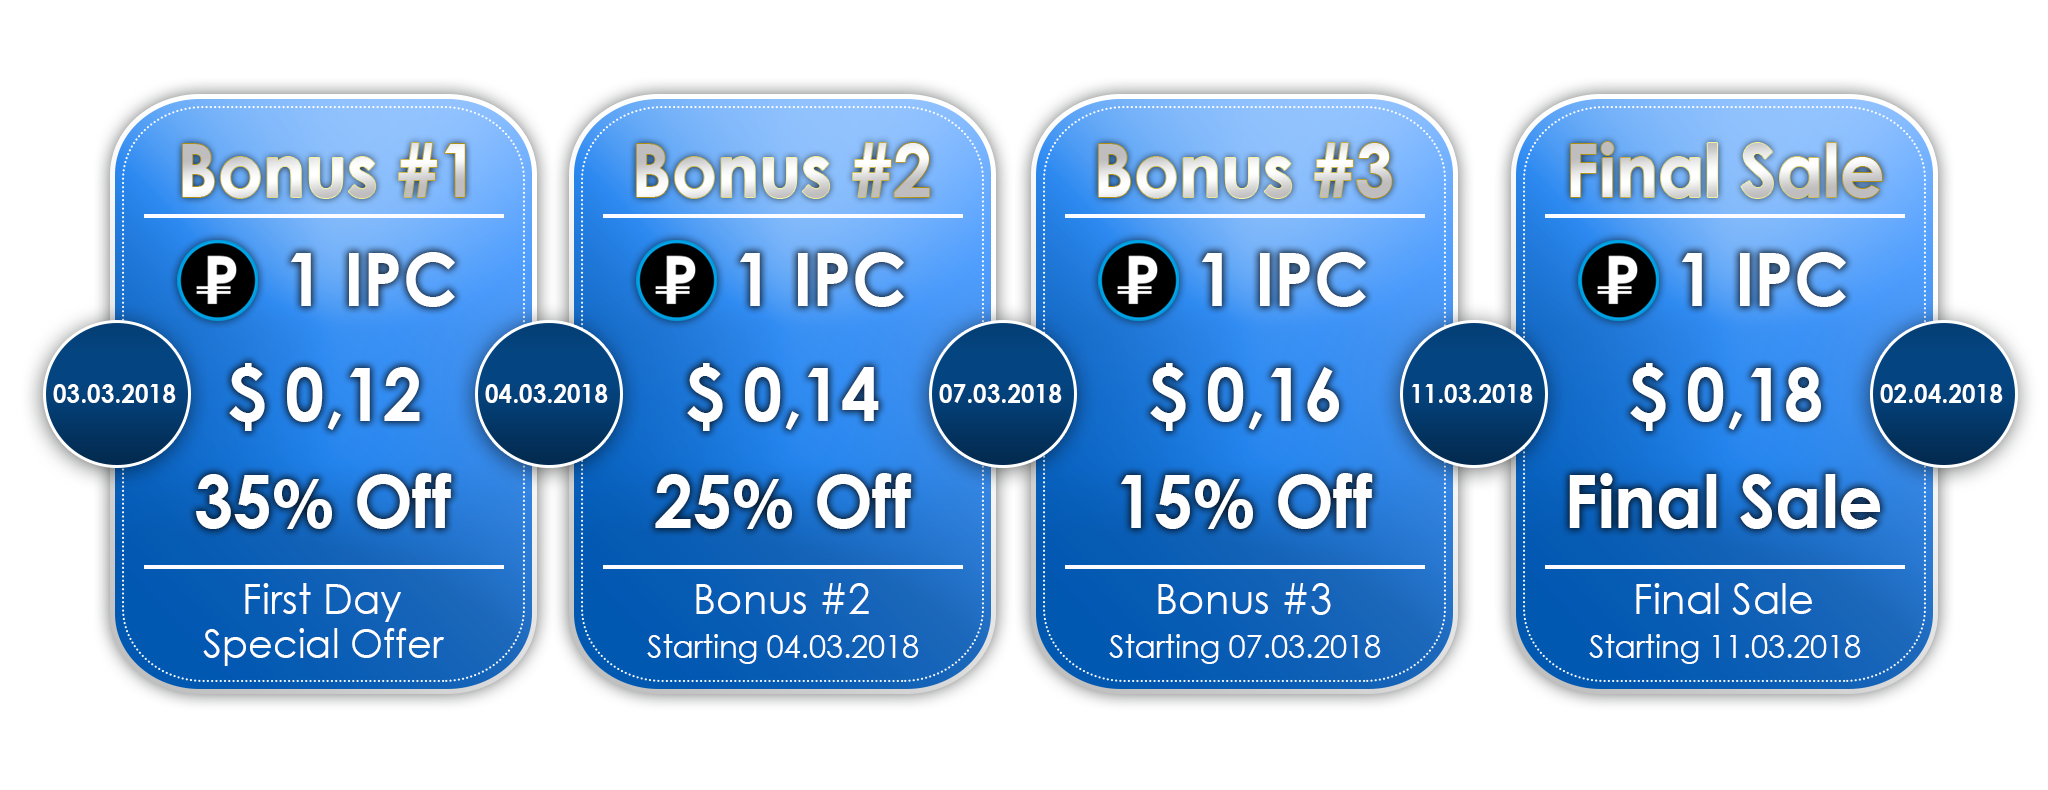
\includegraphics[scale=0.45]{crowdsale.png}
\caption{PAYSURA - Crowdsale Distribution of IPC}
\label{dg1}
\end{figure}
\clearpage

%------------------------------------------------


\section{PAYSURA - The Architecture}

A look at the PAYSURA Development and the Application Architecture (see Figure \ref{fig2}) shows the state-of-the-art PAYSURA technology. The applications of PAYSURA will be implemented with Angular2 using TypeScript and HTML5/CSS3 for a responsive and creative design for a great usability. Angular2 is a modern and very fast framework for web development. Through the lazy loading paradigm, unnecessary modules will only be loaded if they are needed. So even with a poor internet connection the PAYSURA applications will still be fast. 
Angular2 allows a module oriented development and that makes it very scalable. It approaches the performance of applications based on PHP because of the reusable modules developed with typescript and the use of the functionalities of the newest JavaScript version ECMAScript 6. 
\newline Due to the fact that IPC will be a valueable asset and lots of transactions between different users and platforms will take place, a blockchain is the most secure and state-of-the-art technology. There will be multiple writers to modify the database hence not just one transaction can modify the database; one transaction alone will not be able to modify it. To avoid any manipulation of the amount or transfer of the IPC it is necessary to have non-trusting writers on the database. This means that a foreign user can not modify a previously occupied database entry. The confirmation processes will make it possible to create a secure payment system and transaction tracking of the IPC so that no IPC holders face manipulated or false database entries.\\
The graph database Neo4J will be used to store all product information, allowing a fast and comfortable search for the user. Through simple queries and graph processing algorithms, an optimized search and filter can be processed without any long waiting times or other timing issues.\\
This is just a very small look at the development of PAYSURA to get a general understanding that PAYSURA will work only with modern, fast and secure tools.

\begin{figure}[ht]
\centering
\includegraphics[scale=0.5]{architecture.png}
\caption{The PAYSURA Software Architecture}
\label{fig2}
\end{figure}



%------------------------------------------------
\section{PAYSURA - The Roadmap}
PAYSURA's goal is to bring IPC into every use-case a payment transaction is made. Therefore a roadmap containing the first steps is listed below:
\begin{enumerate}

\item	Development of PAYSURA, Prototyping and Concept of PAYSURA
\item	Finding partners and advisors, MVP of Reward Pool
\item	Crowdsale and bringing IPC to the Community
\item	Exchange listing
\item	Wallet for IPC 
\item	Deployment of the reward pool v.1
\item	Registration start on the PAYSURA platform
\item	Publishing New Roadmap

\end{enumerate}
\newpage

\section{PAYSURA - Frequently Asked Questions}

\begin{itemize}
\item What does PAYSURA do in one sentence?
\end{itemize}

PAYSURA is providing the International PayReward Coin (IPC) as a worldwide, uniform reward system that applies the advantages of the blockchain technology to revolutionize the reward systems landscape. 

\begin{itemize}
\item Is PAYSURA a scam?
\end{itemize} 
We are a team consisting of highly motivated university graduates and qualified experts working with private investments dedicated to achieve PAYSURA's mission. All investments taken before the crowdsale are private funds of all PAYSURA team members. The team believes in PAYSURA, by investing large amounts of money and time into the project.


\begin{itemize}
\item Why blockchain?
\end{itemize}

The blockchain is the most secure database for financial assets and perfectly fits the demands of an international reward system. The IPC will be involved in many transactions all over the world. The blockchain as a decentralized data ledger guarantees a non-manipulative system that secures every transaction that is made. Thanks to the blockchain, customers will be able to transfer their IPC to anybody (friends, families or colleagues etc.) in an easy and fast way. 


\begin{itemize}
\item Why is the PAYSURA reward system the better option for customers compared to ordinary reward or loyalty concepts and systems?
\end{itemize}

Traditional reward programs constitue expensive liablilities for merchants without representing a real value for the cutomer. IPC transfers real value to customers, allowing them to use their rewards to purchase new products or services. Due to the fact that the IPC is a token based on theEthereum blockchain, PAYSURA is able to apply the full range of advantages of blockchain technology, creating a cryptocurrency and embedding it into an innovative reward concept.

\begin{itemize}
\item Are there any additional costs for the merchant? What advantages do merchants have from using IPC?
\end{itemize}  
Rather than additional costs, there are less costs for the merchant. Lower costs are primarily possible due to the blockchain and low transaction costs, no accounting overhead costs and automatically regulated reward due to the IPC algorithm. Besides lower costs, IPC and its value as a cryptocurrency goes beyond a reward program, meaning less liability for the merchant.

\begin{itemize}
\item What is it advantage for the customer to use reward in terms of IPC instead of traditional reward programs?
\end{itemize}

- IPC as a Digital Asset \newline
- Secure and global due to blockchain technology \newline
- No expiration date \newline
- International usability \newline
- No physical card \newline
- Flexibility as IPC is transferable to anybody (family, friends, charity) \newline
- Data security (no data vending)\newline


\begin{itemize}
\item What will happen to unsold tokens during the crowdsale?
\end{itemize}
All unsold tokens will be reserved for the community in the reward pool. 




%----------------------------------------------------------------------------------------
%	REFERENCE LIST
%----------------------------------------------------------------------------------------


%----------------------------------------------------------------------------------------

\end{document}
